\chapter{The particle filter}
\label{ch:particle}

The grid of Chapter~\ref{ch:bayes} stored the belief everywhere; the
Kalman filters assumed it was Gaussian. A \emph{particle filter} stores it
as a cloud of weighted samples,
\[
  \bel(\x_t)\approx\sum_{i=1}^Nw_t^{(i)}\,\delta_{\x_t^{(i)}},\qquad
  \sum_iw_t^{(i)}=1,
\]
where $\delta_{\x}$ denotes a point mass at $\x$: the formula says that the
pose is $\x_t^{(i)}$ with probability $w_t^{(i)}$. The average of any
function $\varphi$ of the pose under the belief is then approximated by
the weighted sum $\sum_iw_t^{(i)}\varphi(\x_t^{(i)})$. The filter puts its
effort where the probability is. The cloud can take any shape
(arcs, several separate bumps) and the models are used as they are,
without linearisation; the motion model only needs to be \emph{sampled},
which suits its degenerate transition (\cref{prop:degenerate}). Applied to
robot localisation this is \emph{Monte Carlo localisation}. This chapter
derives it from importance sampling, then studies its three failure
modes---weight degeneracy, sample impoverishment and mode collapse---and
the standard remedies.

\section{Importance sampling}

The particle filter rests on one idea. We want averages under a
distribution $\pi$ (the belief) from which we cannot sample directly, but
we can sample from another distribution $q$. When both have densities,
\[
  \E_\pi[\varphi]=\int\varphi(x)\,\pi(x)\,\mathrm dx
  =\int\varphi(x)\,\frac{\pi(x)}{q(x)}\,q(x)\,\mathrm dx
  =\E_q\Bigl[\varphi\,\frac\pi q\Bigr].
\]
So an average under $\pi$ is an average under $q$ in which each sample $x$
counts with the \emph{weight} $\pi(x)/q(x)$: more where $q$ proposes too
rarely, less where it proposes too often. In a filter, $\pi$ is known only
up to its normalising constant (the $\eta$ of \cref{thm:bayes}); dividing
the weights by their sum removes the need for it.

\begin{example}{Two outcomes}{istwo}
A target gives probability $0.2$ to $a$ and $0.8$ to $b$; the proposal
gives $0.5$ to each. The weights are $\pi/q=0.4$ for $a$ and $1.6$ for $b$.
Let $\varphi(a)=0$ and $\varphi(b)=10$, so that $\E_\pi[\varphi]=8$.
Suppose ten draws from the proposal give $a$ six times and $b$ four times.
The plain average of $\varphi$ over the draws is $4$, far from $8$. The
weights of the ten draws sum to $6\times0.4+4\times1.6=8.8$, and the
weighted average, with the weights divided by their sum, is
$(4\times1.6\times10)/8.8=7.3$: the weights have corrected
most of the mismatch between proposal and target, and the rest is sampling
noise, which vanishes as the number of draws grows.
\end{example}

\Cref{fig:importance} shows the same idea with continuous distributions.
The definition below is stated for general distributions; with densities,
$\mathrm d\pi/\mathrm dq$ is simply the ratio $\pi(x)/q(x)$.

\begin{definition}{Importance sampling}{is}
Let $\pi$ be a target distribution and $q$ a \emph{proposal} with
$\pi\ll q$ (every set of $q$-probability zero has $\pi$-probability
zero), and let $\tilde w=\mathrm d\pi/\mathrm dq$ be known up to a
constant: $\tilde w\propto w$. With $X^{(1)},\dots,X^{(N)}$ drawn
independently from $q$, the \emph{self-normalised} importance-sampling estimate of
$\E_\pi[\varphi]$ is
\[
  \hat\varphi_N=\sum_{i=1}^Nw^{(i)}\varphi(X^{(i)}),\qquad
  w^{(i)}=\frac{w(X^{(i)})}{\sum_kw(X^{(k)})}.
\]
\end{definition}

\begin{proposition}{Consistency}{isconsistent}
If $\E_\pi|\varphi|<\infty$, then $\hat\varphi_N\to\E_\pi[\varphi]$
almost surely as $N\to\infty$. If the normalising constant is known, the
unnormalised estimate $\frac1N\sum_i\tilde w(X^{(i)})\varphi(X^{(i)})$ is
moreover unbiased.
\end{proposition}

\begin{proof}
Write $w=c\,\tilde w$ for an unknown $c>0$. Then
$\E_q[\tilde w\varphi]=\int\varphi\,\frac{\mathrm d\pi}{\mathrm dq}\,
\mathrm dq=\E_\pi[\varphi]$, which is the unbiasedness claim, and
$\E_q[\tilde w]=\int\frac{\mathrm d\pi}{\mathrm dq}\,\mathrm dq=1$ (the
total probability of $\pi$). Both $\tilde w\varphi$ and $\tilde w$ have
finite means under $q$, since $\E_q|\tilde w\varphi|=\E_\pi|\varphi|$.
By the strong law of large numbers applied to the numerator and the
denominator,
\[
  \hat\varphi_N=\frac{\frac1N\sum_i\tilde w(X^{(i)})\varphi(X^{(i)})}
  {\frac1N\sum_i\tilde w(X^{(i)})}\longrightarrow
  \frac{\E_\pi[\varphi]}{1}\quad\text{a.s.,}
\]
the constant $c$ cancelling in the ratio.
\end{proof}

\begin{figure}[ht]
\centering
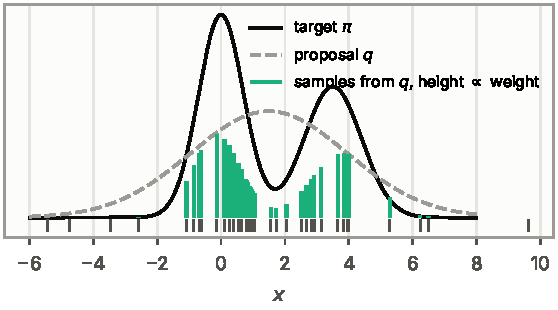
\includegraphics[width=0.75\linewidth]{figures/ch06_importance.pdf}
\caption{Importance sampling. Forty samples are drawn from a wide proposal
$q$ (dashed); each is weighted by $\pi/q$, so that the weighted samples
(green, height proportional to the weight) represent the bimodal target
$\pi$. Samples where $q$ over-represents $\pi$ get small weights.}
\label{fig:importance}
\end{figure}


The self-normalised estimate is
biased for finite $N$
(Exercise~\ref{ex:isbias}), but the bias is $O(1/N)$ and vanishes as $N$
grows (a second-order expansion of the ratio; not proved here, see Doucet
and Johansen in the references).

\section{From the Bayes filter to particles}

The two steps of the Bayes filter translate directly into operations on a
cloud of particles. Suppose the particles $\x_t^{(i)}$, with weights
$w_t^{(i)}$, represent the belief $\bel(\x_t)$.
\begin{itemize}[nosep]
  \item \emph{Predict.} The predicted belief is the distribution of the
    next pose when the current pose is drawn from the belief and one noisy
    step is taken. So take one noisy step from each particle: draw a
    control noise and apply the motion model. The moved particles, with
    the same weights, represent $\belbar(\x_{t+1})$.
  \item \emph{Update.} The new belief is the predicted belief multiplied
    by the likelihood, $\bel\propto p(\z_{t+1}\mid\x)\,\belbar$. This is
    importance sampling with the predicted belief as proposal and the new
    belief as target: the weight of a sample is the ratio of the two,
    which is the likelihood. So multiply the weight of each particle by
    the likelihood of the measurement at that particle, and normalise.
\end{itemize}
\Cref{fig:pfcycle} shows one such cycle on the one-dimensional example of
\cref{fig:bayescycle}, with a third operation, resampling, that is
explained below. The rest of this section makes the argument precise and
states the algorithm.

\begin{figure}[ht]
\centering
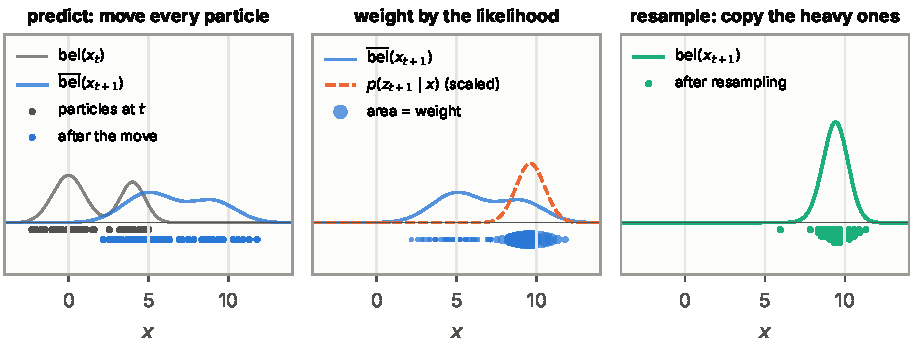
\includegraphics[width=\linewidth]{figures/ch06_pf_cycle.pdf}
\caption{One cycle of a particle filter with $60$ particles, on the example of
\cref{fig:bayescycle}: a two-bump belief, a commanded displacement of $5$
with motion noise, and a measurement whose likelihood peaks at $9.6$. The
curves are the exact
densities computed there: the belief at $t$ (grey), the predicted belief
(blue), the likelihood (dashed) and the new belief (green). Left: each particle (grey dots) is moved by the
commanded displacement plus its own random noise (blue dots). Middle:
each moved particle is weighted by the likelihood of the measurement
(dashed); the area of a dot shows its weight. Right: resampling keeps
$60$ particles of equal weight, by copying the heavy ones (copies are
stacked) and dropping the light ones.}
\label{fig:pfcycle}
\end{figure}

For the precise argument, take the target to be the posterior over the
whole path,
$\pi_t(\x_{0:t})=p(\x_{0:t}\mid\z_{1:t},\uu_{0:t-1})$. It is proportional
to the joint distribution of \cref{prop:joint}, and going from $t$ to
$t+1$ multiplies it by one motion factor and one measurement
factor. So
$\pi_{t+1}(\x_{0:t+1})\propto\pi_t(\x_{0:t})\,p(\x_{t+1}\mid\x_t,\uu_t)\,
p(\z_{t+1}\mid\x_{t+1})$. Choose as proposal ``the previous proposal,
extended by the motion model'':
$q_{t+1}(\x_{0:t+1})=q_t(\x_{0:t})\,p(\x_{t+1}\mid\x_t,\uu_t)$.

\begin{proposition}{Sequential importance sampling with the motion proposal}{sis}
With this proposal, the weights obey
\[
  \tilde w_{t+1}(\x_{0:t+1})\propto\tilde w_t(\x_{0:t})\;
  p(\z_{t+1}\mid\x_{t+1}).
\]
\end{proposition}

\begin{proof}
Formally $\tilde w_{t+1}=\pi_{t+1}/q_{t+1}$, and the factor
$p(\x_{t+1}\mid\x_t,\uu_t)$ appears in both and cancels:
$\tilde w_{t+1}\propto\frac{\pi_t}{q_t}\,p(\z_{t+1}\mid\x_{t+1})$.

This factor is the transition, a distribution without a density
(\cref{prop:degenerate}), so the cancellation is not a division of two
functions and deserves a word. A path is drawn from $q_{t+1}$ by drawing
$\x_{0:t}$ from $q_t$ and then $\x_{t+1}$ from the transition. An average
under $\pi_{t+1}$ is obtained, up to a constant, by drawing $\x_{0:t}$ from
$\pi_t$, then $\x_{t+1}$ from the \emph{same} transition, and weighting by
$p(\z_{t+1}\mid\x_{t+1})$. Replacing the draw from $\pi_t$ by a draw from
$q_t$ weighted by $\tilde w_t$, for every function $g$ of the path,
\[
  \E_{\pi_{t+1}}[g]\;\propto\;\E_{q_{t+1}}\bigl[g\;\tilde w_t(\x_{0:t})\,
  p(\z_{t+1}\mid\x_{t+1})\bigr].
\]
This is the statement
$\mathrm d\pi_{t+1}/\mathrm dq_{t+1}\propto\tilde w_t\,
p(\z_{t+1}\mid\x_{t+1})$ of \cref{def:is}. The transition is sampled,
never evaluated.
\end{proof}

\begin{definition}{Particle filter (sequential importance resampling)}{pf}
Given particles and normalised weights $(\x_t^{(i)},w_t^{(i)})$:
\begin{enumerate}[nosep]
\item \emph{Predict}: draw $\bepsilon^{(i)}\sim\Normal(\vect0,M)$ and set
  $\x_{t+1}^{(i)}=f(\x_t^{(i)},\uu_t+\bepsilon^{(i)})$.
\item \emph{Weight}: $w_{t+1}^{(i)}\propto w_t^{(i)}\,
  p(\z_{t+1}\mid\x_{t+1}^{(i)})$, normalised to sum to one.
\item \emph{Resample} if the effective sample size (\cref{def:ess}) drops
  below a threshold: draw $N$ particles from the cloud with probabilities
  $w^{(i)}$, and reset every weight to $1/N$.
\end{enumerate}
The estimate is the weighted mean (with a circular mean for the heading,
\cref{sec:circular})
and the weighted covariance of the cloud.
\end{definition}

The implementation departs from this definition in two ways, both common
in practice. It propagates the particles with a motion noise inflated by
$1.5$ in standard deviation (covariance $2.25M$, option
\code{motion\_inflation}), which keeps the cloud from becoming too
narrow; and it gives the likelihood $0$ to a particle more than 5 units
outside the lawn. With the inflation the filter no longer samples the
exact transition, so its cloud is somewhat wider than the true belief.
All the particle-filter results of this book use these settings.

\begin{inwords}
\emph{Simulate} the motion for every particle, \emph{score} each one
against the measurement, \emph{clone} the good ones and \emph{drop} the
bad ones. That is the whole algorithm. The sensor model is the same as for
the Kalman filters: a product of Gaussians in range and wrapped bearing
over the visible landmarks.
\end{inwords}

\paragraph{Log-weights.} With four precise landmarks, a particle 50 units
from the truth has a likelihood around $e^{-200}$ relative to a good one:
if its four ranges are each off by about $50=10\,\sigma_r$, each
contributes a factor $e^{-10^2/2}=e^{-50}$. The products underflow
quickly. The implementation adds log-likelihoods and normalises with
$\log\sum_ie^{a_i}=a_{\max}+\log\sum_ie^{a_i-a_{\max}}$ (factor
$e^{a_{\max}}$ out of the sum), in which every exponential is at most
$1$ and the largest is exactly $1$. Fixed rescaling factors, or thresholds on raw
weights, break as soon as the number of visible landmarks or the noise
level changes.

\section{Weight degeneracy}

At each update the weights are multiplied by likelihoods, and after a few
updates they become very uneven: a few particles carry almost all the
weight. One number summarises how uneven they are.

\begin{definition}{Effective sample size}{ess}
For normalised weights, $\ESS=1/\sum_i(w^{(i)})^2\in[1,N]$.
\end{definition}

$\ESS=N$ when all the weights are equal and $\ESS=1$ when one particle
carries all the weight (Exercise~\ref{ex:ess}). It approximates the number
of independent samples drawn directly from the target that would give the
same variance (Kong, Liu and Wong, in the references):
a first-order expansion of the ratio that defines $\hat\varphi_N$ (the
delta method), together with the further approximation that the weights
are uncorrelated with $(\varphi-\E_\pi\varphi)^2$, gives
$\Var(\hat\varphi_N)\approx\Var_\pi(\varphi)\,(1+\mathrm{cv}^2)/N$, where $\mathrm{cv}$ is the coefficient of
variation of the unnormalised weights (their standard deviation divided
by their mean), and $N/(1+\mathrm{cv}^2)$ is
estimated by the ESS.

Run without resampling, sequential importance sampling degenerates
quickly (\cref{fig:ess}). Starting from a Gaussian around the truth with
$N=1000$, the ESS falls below $2$ at step 5: one particle carries all the
weight, the other 999 are wasted computation, and the estimate drifts away
with that single survivor. The variance of the unnormalised weights, with
the measurements treated as random, can only grow over time (Kong, Liu
and Wong, 1994); in a given run it can occasionally decrease. Resampling is what makes the method
work.

\begin{figure}[ht]
\centering
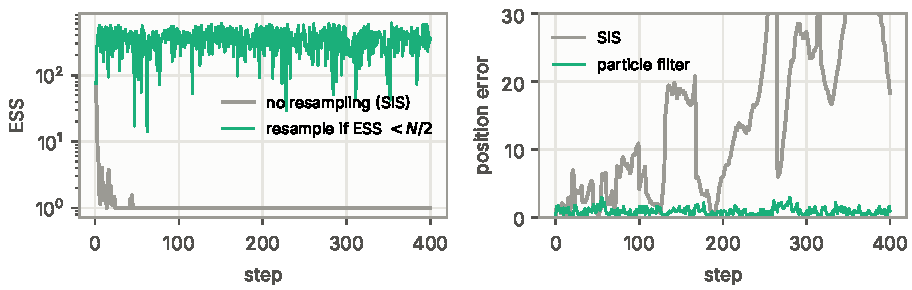
\includegraphics[width=\linewidth]{figures/ch06_ess.pdf}
\caption{Left: ESS before resampling (log scale), $N=1000$. Without
resampling it collapses to 1 within five steps; resampling whenever
$\ESS<N/2$ keeps it in the hundreds. Right: the corresponding position
errors.}
\label{fig:ess}
\end{figure}

\section{Resampling}

Resampling replaces the weighted cloud by an unweighted one that
represents the same belief: it draws $N$ new particles from the old ones,
each old particle being chosen with a probability equal to its weight.
Heavy particles are copied several times, light ones tend to disappear,
and all the new particles get the weight $1/N$ (\cref{fig:pfcycle},
right). The computation is then spent on the particles that matter. The
price is some extra randomness, since the number of copies of each
particle is random, and the way the draw is made decides how much.
\Cref{fig:systematic} shows the method used in this book.

Let $N_i$ be the number of copies of particle $i$ after resampling.
Ideally $N_i$ would be $Nw^{(i)}$, but that is rarely a whole number.

\begin{proposition}{Multinomial and systematic resampling}{resampling}
\emph{Multinomial} resampling draws $N$ indices independently from the
weights.
\emph{Systematic} resampling draws one $U\sim\mathcal U[0,1)$ and selects
the particles whose cumulative-weight intervals contain the $N$ points
$(U+k)/N$, $k=0,\dots,N-1$. Both are unbiased, $\E[N_i]=Nw^{(i)}$, and
\begin{align*}
  \text{multinomial:}&\quad N_i\sim\operatorname{Bin}(N,w^{(i)}),
  &\Var(N_i)&=Nw^{(i)}(1-w^{(i)}),\\
  \text{systematic:}&\quad N_i\in\{\lfloor Nw^{(i)}\rfloor,
  \lceil Nw^{(i)}\rceil\},&\Var(N_i)&=f_i(1-f_i)\le\tfrac14,
\end{align*}
where $f_i=Nw^{(i)}-\lfloor Nw^{(i)}\rfloor$.
\end{proposition}

\begin{proof}
Multinomial: each draw selects $i$ with probability $w^{(i)}$,
independently, so $N_i$ counts the successes of $N$ independent trials of
probability $w^{(i)}$. Systematic: particle $i$ owns an interval $I_i$ of
length $w^{(i)}$ in $[0,1)$, and the points $(U+k)/N$ form a lattice of
spacing $1/N$ with a uniformly random offset. An interval of length
$\ell$ spans $N\ell$ spacings, so it contains at least $\lfloor
N\ell\rfloor$ and at most $\lceil N\ell\rceil$ lattice points. For the
mean: the point $(U+k)/N$ is uniform on $[k/N,(k+1)/N)$, so it falls in
$I_i$ with probability $N\,\abs{I_i\cap[k/N,(k+1)/N)}$; summing over $k$,
$\E[N_i]=N\abs{I_i}=Nw^{(i)}$. A variable
taking the values $m$ and $m+1$ with mean $m+f_i$ takes $m+1$ with
probability $f_i$, hence the variance $f_i(1-f_i)$.
\end{proof}

\begin{figure}[ht]
\centering
\begin{tikzpicture}[x=11cm,y=1cm,>=Stealth]
  \def\ws{0.08,0.30,0.05,0.12,0.25,0.20}
  \def\cols{{"blue!25","orange!35","green!30","violet!25","teal!25",
    "red!20"}}
  \pgfmathsetmacro{\U}{0.06}
  \foreach \w [count=\i from 0, remember=\c as \cprev (initially 0)] in \ws {
    \pgfmathsetmacro{\c}{\cprev+\w}
    \pgfmathsetmacro{\col}{\cols[\i]}
    \fill[\col] (\cprev,0) rectangle (\c,0.5);
    \draw[black!60] (\cprev,0) rectangle (\c,0.5);
    \pgfmathtruncatemacro{\k}{\i+1}
    \node[font=\scriptsize] at ({(\cprev+\c)/2},0.25) {$w^{(\k)}$};
  }
  \draw[->,black!60] (0,-0.2) -- (1.03,-0.2);
  \node[below,font=\scriptsize] at (0,-0.2) {$0$};
  \node[below,font=\scriptsize] at (1,-0.2) {$1$};
  \foreach \k in {0,...,5} {
    \pgfmathsetmacro{\pos}{(\U+\k)/6}
    \draw[->,thick,black!85] (\pos,1.25) -- (\pos,0.55);
  }
  \pgfmathsetmacro{\pfirst}{\U/6}
  \pgfmathsetmacro{\psecond}{(\U+1)/6}
  \node[above,font=\scriptsize] at (\pfirst,1.25) {$U/N$};
  \node[above,font=\scriptsize] at (\psecond,1.25) {$(U+1)/N$};
  \node[above,font=\scriptsize] at (0.75,1.25) {$\dots$ spacing $1/N$};
\end{tikzpicture}
\caption{Systematic resampling with $N=6$. The weights are laid end to end
on $[0,1)$; one uniform offset $U$ fixes $N$ evenly spaced pointers, and
each particle is copied once per pointer that falls in its interval. Here
particle 2 gets two copies, particles 1, 4, 5 and 6 one each, and particle
3 none: always $\lfloor Nw^{(i)}\rfloor$ or $\lceil Nw^{(i)}\rceil$ (the
expected numbers are $0.48$, $1.8$, $0.3$, $0.72$, $1.5$, $1.2$).}
\label{fig:systematic}
\end{figure}

\begin{figure}[ht]
\centering
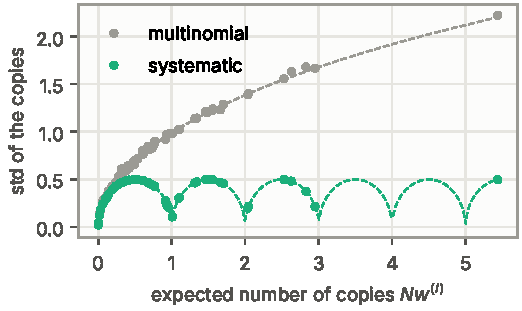
\includegraphics[width=0.62\linewidth]{figures/ch06_resampling.pdf}
\caption{Standard deviation of the number of copies, for 50 particles
and 2\,000 repetitions; dashed lines: the formulas of
\cref{prop:resampling}. Systematic resampling adds almost no noise.}
\label{fig:resampling}
\end{figure}

Each resampling destroys diversity: duplicated particles are identical
until the motion noise separates them. Resampling at every step is
therefore unnecessary and harmful. The filter here resamples only when
$\ESS<N/2$. With four precise landmarks that is still 85\% of the steps,
because each measurement is very informative compared with one step of
motion noise.

On the standard run, with a good initial estimate and identified
landmarks, the particle filter with $N=1000$ has an RMSE of $1.02$,
against $1.01$ for the EKF, at about eight times the cost per step. When
the belief is close to a Gaussian, the particle filter has nothing to add.

\section{Global localisation and sample impoverishment}
\label{sec:global}

A Kalman filter needs an initial guess. A particle filter can start from a
\emph{uniform} belief over the whole lawn and every heading.

\begin{figure}[ht]
\centering
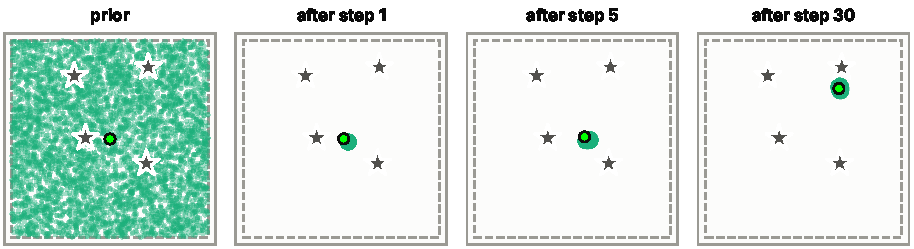
\includegraphics[width=\linewidth]{figures/ch06_global.pdf}
\caption{Global localisation with $N=5000$ (green dot: the robot). One
measurement leaves essentially one compatible particle. After
resampling, all 5\,000 particles are its copies, and the motion noise
slowly spreads them onto the robot.}
\label{fig:global}
\end{figure}

After the first measurement the ESS is $1.0$ out of $5\,000$
(\cref{fig:global}). The reason is a matter of volumes. The prior covers
$320\times320\times2\pi\approx6\times10^5$ units of pose space. After
four ranges and four bearings the posterior has standard deviations of
about $2.6$ and $1.6$ in position and $0.026$\,rad in heading (the
information form of \cref{prop:information}, evaluated at the start
pose; notebook~05 computes them): a box of volume $2.6\times1.6\times0.026\approx0.1$. A uniform
particle falls in that box with probability $0.1/(6\times10^5)\approx
2\times10^{-7}$, so the expected number of particles inside it is about
$2N\times10^{-7}$: far below one for any affordable $N$. The best particle
is a few units from the truth, and the filter must then crawl to it
through the motion noise. This is \emph{sample impoverishment}: the
posterior is much narrower than the spacing between the particles.

\begin{inwords}
Particles are only useful where the probability is, and when the
likelihood is sharp, ``where the probability is'' is a tiny region that a
uniform cloud almost never hits. More particles help only slowly; in
higher dimensions the volume ratio explodes, which is the particle
filter's real weakness.
\end{inwords}

The remedies all widen the effective likelihood or move particles
towards it: \emph{roughening} (a small jitter after resampling), a
\emph{tempered} likelihood $p(\z\mid\x)^\beta$ with $\beta<1$ for the
first updates, or \emph{sensor resetting}, which draws some particles
directly from the poses compatible with the measurement.

\section{Unknown data association and multimodal beliefs}
\label{sec:pf-association}

When the sensor does not say which landmark it saw, the likelihood of one
measurement is a mixture over the landmarks that could have produced it:
\[
  p(\z_k\mid\x)=\frac1{n_\ell}\sum_{j=1}^{n_\ell}\Normal\bigl(\z_k;\,
  h_j(\x),\,R_1\bigr),
\]
assuming each landmark equally likely a priori. A particle filter simply
evaluates it: every particle is scored against every possible
association, and no decision is ever taken. Attributing each measurement
to the nearest landmark, as an EKF must, amounts to replacing the sum by
its largest term.

Take a different world for this experiment: four landmarks on a square,
at $(\pm80,\pm80)$. The lawn is then symmetric under rotations by
$90^\circ$ and, without identities, four poses explain the
measurements equally well forever. The true posterior has four bumps of
mass $1/4$ each. \Cref{fig:modes} shows what the particle filter does with
it (the noise is raised to $\sigma_r=15$ and $\sigma_\phi=0.25$, so that
$20\,000$ particles resolve all four modes from a uniform start).

\begin{figure}[ht]
\centering
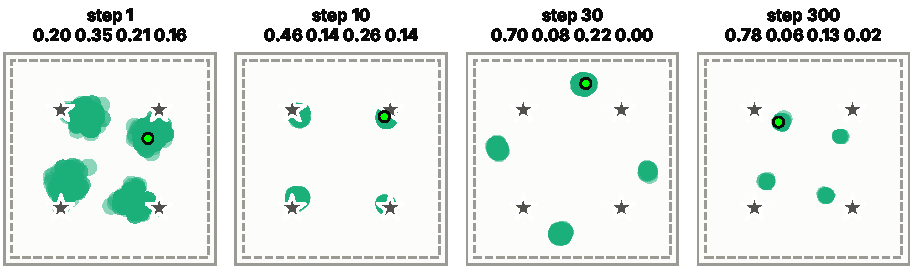
\includegraphics[width=\linewidth]{figures/ch06_modes.pdf}
\caption{Symmetric landmarks, unknown identities, $N=20\,000$. Above each
panel: the mass of the four modes (rotations of the true pose). The
correct posterior has four masses of $0.25$ forever; the particle
estimates drift.}
\label{fig:modes}
\end{figure}

The cloud correctly splits into four clusters. But the masses
($0.20$, $0.35$, $0.21$, $0.16$ after one step) drift: after 30 steps one
mode holds $0.70$ and another $0.005$ (notebook~05 prints them), fewer than a hundred particles. A
mode that loses its last particle never comes back. With fewer particles
it happens much sooner: with $N=2000$ only one mode is left by step 30 in
each of three runs.

The drift has a simple explanation, which needs one notion. A
\emph{martingale} is a random process whose expected next value, given its
present value, is the present value: it has no tendency to go up or down,
but it does fluctuate.

\begin{proposition}{Mode masses are martingales with absorbing ends}{wrightfisher}
Idealise the situation: two modes $A$ and $B$ whose particles all have
the same likelihood, so that the weights stay equal, and multinomial
resampling at every step. Let
$m_t$ be the fraction of particles in $A$. Then $(m_t)$ is a martingale,
$\E[m_{t+1}\mid m_t]=m_t$ and $\Var(m_{t+1}\mid m_t)=m_t(1-m_t)/N$. It
reaches $0$ or $1$ in finite time with probability one, and reaches $1$
with probability $m_0$.
\end{proposition}

\begin{proof}
After resampling, the number of particles in $A$ is
$\operatorname{Bin}(N,m_t)$ (each draw lands in $A$ with probability
$m_t$), so $Nm_{t+1}$ has mean $Nm_t$ and variance $Nm_t(1-m_t)$;
dividing by $N$ and $N^2$ gives the mean and variance of $m_{t+1}$.

\emph{Absorption.} The states $0$ and $1$ are absorbing: an empty mode
receives no draws, and a full one receives all of them. From any other
state $m$, all $N$ draws miss $A$ with probability $(1-m)^N>0$; over the
finitely many states $k/N$, $0<k<N$, this probability is at least some
$c>0$. So the probability of not being absorbed during $k$ steps is at
most $(1-c)^k\to0$: absorption happens with probability one, at a random
time $\tau$.

\emph{Where it ends.} Taking expectations in $\E[m_{t+1}\mid m_t]=m_t$
gives $\E[m_{t+1}]=\E[m_t]$, so $\E[m_t]=m_0$ for every $t$. After $\tau$
the fraction no longer changes, so $m_t\to m_\tau$ with probability one;
$0\le m_t\le1$, so dominated convergence gives $\E[m_\tau]=m_0$. Since
$m_\tau\in\{0,1\}$, $\E[m_\tau]=\Pr(m_\tau=1)$, which is therefore $m_0$.
\end{proof}

\begin{inwords}
This is the neutral Wright--Fisher model of population genetics: genetic
drift. Without any evidence favouring one mode, the particle population
still ``chooses'' one at random, and the filter ends up claiming a
certainty that the data do not support. The proposition isolates the
noise of resampling. In \cref{fig:modes} the weighting step adds a
larger Monte Carlo noise of its own: with random weights, the variance
per step gains a term from the spread of the weight of each mode, and the
drift is much faster than the resampling noise alone would give
(Exercise~\ref{ex:fixation} predicts about $1\,400$ resamplings to halve
the spread of a $50/50$ split with $N=2000$, against one mode left by step
30 in the runs above). Systematic resampling reduces the resampling noise,
but not the weighting noise, so the drift remains. More particles slow it down
(the variance per step is $\propto1/N$); nothing stops it. The weighted
mean is meaningless here; a multimodal belief should be reported by its
modes.
\end{inwords}

\section{The kidnapped robot}
\label{sec:amcl}

\emph{Kidnapped} is the standard name in robotics (the \emph{kidnapped
robot problem}) for a robot that is picked up and moved somewhere else
without being told: someone lifts the robot and puts it down on another
part of the lawn. The filter keeps receiving ordinary commands and
measurements, and nothing tells it that the robot has moved. This is
harder than global localisation: there the filter \emph{knows} that it does
not know where the robot is; here it is \emph{confidently wrong}, and must
first discover that its belief is wrong. A converged particle filter has
no particles near the new pose, so it can only crawl there through the
motion noise, if at all.

The way to discover it is \cref{prop:evidence}: the normaliser of the
Bayes filter is the predictive likelihood of the measurement, and a
kidnapping makes it collapse.

\begin{proposition}{Estimating the predictive likelihood}{avglik}
Let $(\x^{(i)},w^{(i)})$ be the predicted cloud, approximating
$\belbar(\x_{t+1})$. Then
\[
  \hat\ell_{t+1}=\sum_iw^{(i)}\,p(\z_{t+1}\mid\x^{(i)})
  \longrightarrow\int p(\z_{t+1}\mid\x)\,\belbar(\x)\,\mathrm d\x=
  \eta_{t+1}^{-1}
\]
as $N\to\infty$, assuming that the predicted cloud is a consistent
approximation of $\belbar$.
\end{proposition}

\begin{proof}
For independent draws from a fixed proposal this is
\cref{prop:isconsistent} with $\varphi(\x)=p(\z_{t+1}\mid\x)$, which is
bounded, and the target $\belbar$; the identification of the limit is
\cref{prop:evidence}. A resampled and propagated cloud is not a set of
independent draws, and its consistency is a theorem of its own, not proved
here (see Doucet and Johansen in the references).
\end{proof}

The idea of \emph{augmented} Monte Carlo localisation is to watch this
number over time. While the filter is tracking, the measurements are
explained about as well as usual. After a kidnapping they are suddenly
explained much worse than usual. ``Usual'' is measured by a long-term
average of $\hat\ell_t$, and ``now'' by a short-term one. Both are
\emph{exponential averages}: at each step the average moves a fraction
$\alpha$ of the way towards the new value, so that a small $\alpha$ gives
a long memory and a large $\alpha$ a short one.

\begin{definition}{Augmented MCL}{amcl}
Maintain two exponential averages of $\hat\ell_t$, a slow one and a fast
one ($0<\alpha_{\mathrm{slow}}\ll\alpha_{\mathrm{fast}}<1$):
\[
  w_{\mathrm{slow}}\leftarrow w_{\mathrm{slow}}+\alpha_{\mathrm{slow}}
  (\hat\ell_t-w_{\mathrm{slow}}),\qquad
  w_{\mathrm{fast}}\leftarrow w_{\mathrm{fast}}+\alpha_{\mathrm{fast}}
  (\hat\ell_t-w_{\mathrm{fast}}),
\]
and, whenever $p=\max(0,1-w_{\mathrm{fast}}/w_{\mathrm{slow}})$ is
positive, resample and replace each particle, with probability $p$, by a
pose drawn uniformly over the lawn.
\end{definition}

When the measurements suddenly become hard to explain, the fast average
drops below the slow one, and a fraction of the particles is scattered
over the lawn; some land near the new pose and are quickly amplified by
the next updates. While tracking normally, $w_{\mathrm{fast}}$ stays
above $w_{\mathrm{slow}}$ and nothing is injected. (In \cref{fig:amcl} it
is about six times above, because both start from the first value of
$\hat\ell$, after the global start, and $w_{\mathrm{slow}}$ still
remembers those low values.) \Cref{fig:amcl} shows the mechanism on one
kidnapping.

\begin{figure}[ht]
\centering
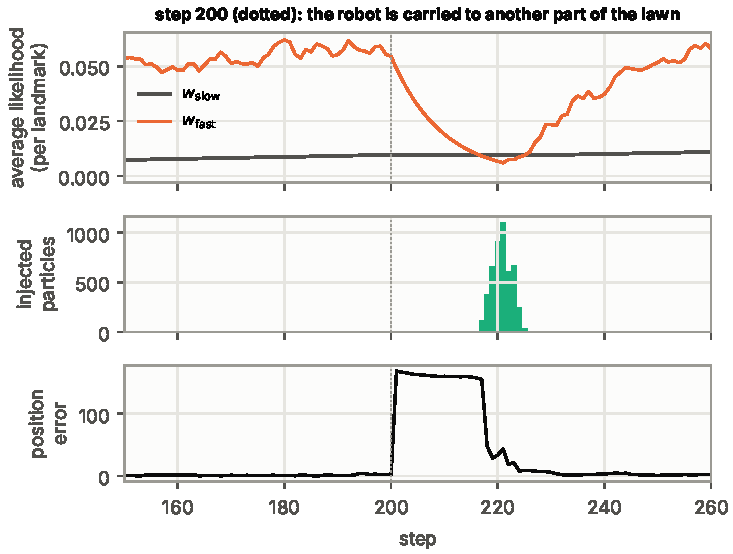
\includegraphics[width=0.8\linewidth]{figures/ch06_amcl.pdf}
\caption{Augmented MCL around the kidnapping of \cref{fig:kidnap}: at step $200$
(dotted) the robot is carried to another part of the lawn (unknown
landmark identities, $N=3000$). Top: after the kidnapping the measurement likelihood is
close to zero, so the fast average decays by the factor
$1-\alpha_{\mathrm{fast}}=0.9$ per step; the slow one barely moves. Middle: once
$w_{\mathrm{fast}}<w_{\mathrm{slow}}$ (step 217), random particles are
injected. Bottom: some of them land near the new pose, and the position
error drops back to a few units.}
\label{fig:amcl}
\end{figure}

The implementation averages the \emph{per-landmark} likelihood (the
geometric mean over the visible landmarks, $\hat\ell_t^{1/m}$), so that
the scale of $\hat\ell$ does not jump when the number of visible landmarks
changes.

\begin{figure}[ht]
\centering
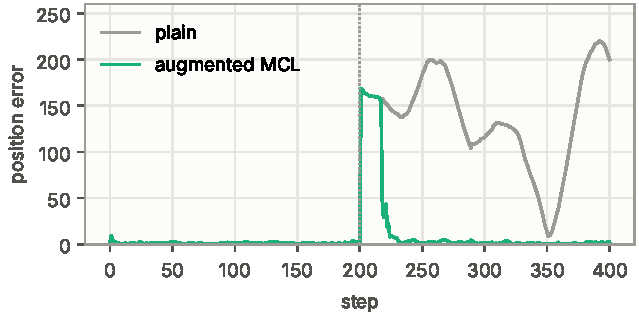
\includegraphics[width=0.75\linewidth]{figures/ch06_kidnap.pdf}
\caption{Kidnapped at step 200 (dotted line), unknown landmark identities,
$N=3000$, seed 7. Without injection the filter does not find the robot
again: its error dips briefly around step 350 and grows back. With
augmented MCL it recovers within about 25 steps and stays locked.}
\label{fig:kidnap}
\end{figure}

Over eight kidnappings (unknown identities, $N=3000$), the number of steps
until the error stays below 10 is $20$ to $41$ with augmented MCL.
Without it, four of the eight runs never recovered within 200 steps, and
the other four took $51$ to $113$ steps (the run of \cref{fig:kidnap} is
one of the eight). All the kidnapping runs use a roughening of $0.5$
(below).

\begin{practice}[\nb{05\_particle\_filter.ipynb}, \code{pf.py}]
\code{ParticleFilter} stores the particles as an $(N,3)$ array and the
log-weights as an $N$-vector. Options: \code{init="global"} or a Gaussian;
\code{association="known"} or \code{"unknown"} (the mixture likelihood);
\code{resample\_threshold} (on $\ESS/N$); \code{systematic\_resample} or
\code{multinomial\_resample}; \code{roughening}; and
\code{recovery=(alpha\_slow, alpha\_fast)} for augmented MCL. The filter
records its ESS, resampling and injection history. The notebook reproduces
\cref{fig:ess,fig:resampling,fig:global,fig:modes,fig:kidnap} and counts
the surviving modes for several $N$; the other figures are produced by
\code{book/figures/make\_figures.py}.
\end{practice}

\begin{mower}
Robot mowers are kidnapped all the time: carried to another part of the
garden, lifted by a curious child, or simply switched off in the shed and
on again on the lawn. Most have a lift sensor, which tells the filter that
a kidnapping happened and lets it re-initialise globally. Augmented MCL
covers the cases a lift sensor misses, such as wheels sliding on a wet
slope.
\end{mower}

\section*{What to remember from this chapter}
\addcontentsline{toc}{section}{What to remember}

\begin{enumerate}[nosep]
  \item A particle filter represents the belief by weighted samples. One
    cycle: move every particle with the noisy motion model, multiply its
    weight by the likelihood of the measurement, and resample when the
    weights become too uneven.
  \item It is importance sampling applied step by step, with the motion
    model as proposal; the motion model is only sampled, never evaluated.
  \item Without resampling the weights degenerate: one particle ends up
    with all the weight. The effective sample size measures this, and
    systematic resampling is the low-noise way to resample.
  \item The filter can start from a uniform belief and handle unknown
    landmark identities and several hypotheses, which the Kalman filters
    cannot.
  \item Its weaknesses are sample impoverishment (a sharp likelihood that
    no particle hits), the random loss of modes, and a cost that grows
    quickly with the dimension of the state.
  \item A kidnapped robot is detected by the collapse of the measurement
    likelihood; augmented MCL then injects random particles.
\end{enumerate}

\FloatBarrier
\section*{Exercises}
\addcontentsline{toc}{section}{Exercises}

\begin{enumerate}[label=\textbf{6.\arabic*},ref=6.\arabic*]
\item\label{ex:ess} Show that $1\le\ESS\le N$, with equality on the right
  if and only if all weights are equal and on the left if and only if one
  weight is $1$. Show that $\ESS=N/(1+N^2s^2)$, where $s^2$ is the
  empirical variance of the normalised weights.
\item\label{ex:isbias} Let the target be $\pi=\Normal(1,1)$, the proposal
  $q=\Normal(0,1)$ and $\varphi(x)=x$. For $N=1$, what does the
  self-normalised estimate return, and what is its mean? Conclude that it
  is biased.
\item\label{ex:stratified} \emph{Stratified} resampling draws one
  independent uniform in each $[k/N,(k+1)/N)$ instead of one shared
  offset. Show that it is unbiased and that $\Var(N_i)\le Nw^{(i)}
  (1-w^{(i)})$ for every $i$.
\item\label{ex:fixation} In \cref{prop:wrightfisher}, show that
  $\E[m_{t}(1-m_{t})]=m_0(1-m_0)(1-1/N)^t$. After how many resamplings
  has the ``heterozygosity'' of a $50/50$ split dropped by half, for
  $N=2000$?
\end{enumerate}

\subsection*{Solutions}

\solution{6.1} With $\sum_iw_i=1$ and $w_i\ge0$, $\sum_iw_i^2\le
\sum_iw_i\max_kw_k\le1$, with equality iff one weight is $1$. By
Cauchy--Schwarz, $1=(\sum_iw_i)^2\le N\sum_iw_i^2$, with equality iff all
the weights are equal. The empirical mean of the weights is $1/N$, so
$s^2=\frac1N\sum_iw_i^2-\frac1{N^2}$, i.e.\ $\sum_iw_i^2=Ns^2+1/N$ and
$\ESS=1/(Ns^2+1/N)=N/(1+N^2s^2)$.

\solution{6.2} With one sample the normalised weight is $1$, so
$\hat\varphi_1=X^{(1)}$, whose mean under $q$ is $0$, not $\E_\pi[X]=1$.
The ratio of two unbiased estimates is not unbiased; the bias of the
self-normalised estimate shrinks like $1/N$.

\solution{6.3} The pointer $U_k\sim\mathcal U[k/N,(k+1)/N)$ falls in
particle $i$'s interval $I_i$ with probability $N|I_i\cap[k/N,
(k+1)/N)|=:p_{ik}$, so $\E[N_i]=\sum_kp_{ik}=N|I_i|=Nw^{(i)}$. The
pointers are independent, so $N_i$ is a sum of independent Bernoulli
variables with parameters $p_{ik}$ and
$\Var(N_i)=\sum_kp_{ik}(1-p_{ik})$. For a fixed sum $\sum_kp_{ik}=
Nw^{(i)}$, $\sum_kp_{ik}^2\ge(\sum_kp_{ik})^2/N=Nw^{(i)2}$ by
Cauchy--Schwarz, so $\Var(N_i)\le Nw^{(i)}-Nw^{(i)2}$.

\solution{6.4} Let $h_t=m_t(1-m_t)$. Given $m_t$,
$\E[m_{t+1}^2]=\E[m_{t+1}]^2+\Var(m_{t+1})=m_t^2+m_t(1-m_t)/N$, so
\[
  \E[h_{t+1}\mid m_t]=\E[m_{t+1}]-\E[m_{t+1}^2]
  =m_t-m_t^2-\frac{m_t(1-m_t)}N=h_t\Bigl(1-\frac1N\Bigr).
\]
Taking expectations, $\E[h_{t+1}]=(1-1/N)\,\E[h_t]$, and after $t$ steps
$\E[h_t]=(1-1/N)^th_0$. For $N=2000$,
$(1-1/N)^t=1/2$ gives $t=\log2/(-\log(1-1/2000))\approx1386$
resamplings: slow, but certain, and faster with fewer particles or
noisier weights.
